\section{Ejercicio 6 - Proporcionar nombres de miembros de dimensión únicos}  

1. Haga clic en la carpeta Vistas del origen de datos en el Explorador de soluciones, después haga doble clic en el
origen de datos Adventure Works DW2012.dsv

2. En el panel Tablas, haga clic derecho en DimDate y, a continuación, haga clic en Nuevo cálculo con nombre

3. En el cuadro de diálogo Crear cálculo con nombre, escriba MonthName en el cuadro Nombre de columna y, a
continuación, escriba la siguiente instrucción en el cuadro Expresión:

	\begin{center}
	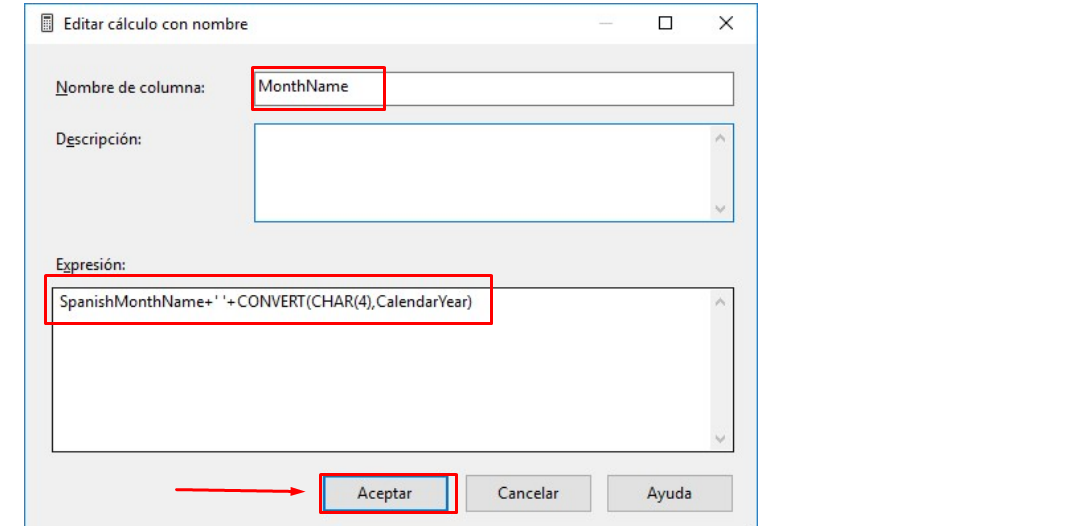
\includegraphics[width=\columnwidth]{images/task6/img1}
	\end{center}	

4. Esta instrucción concatena el mes y el año de cada mes de la tabla a una nueva columna.

5. Haga clic en Aceptar

6. En el panel Tablas, haga clic derecho DimDate y, a continuación, haga clic en Nuevo cálculo con nombre

7. En el cuadro de diálogo Crear cálculo con nombre, escriba CalendarQuarterDesc en el cuadro Nombre de
columna y, a continuación, escriba el script SQL siguiente en el cuadro Expresión:

	\begin{center}
	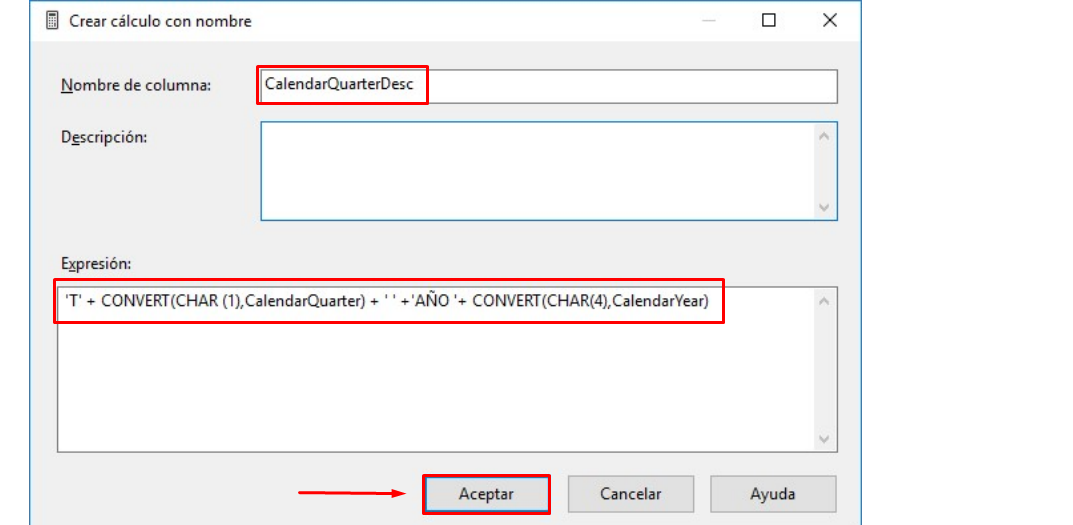
\includegraphics[width=\columnwidth]{images/task6/img2}
	\end{center}	

8. Este script SQL concatena el trimestre natural y el año de cada trimestre de la tabla en una nueva columna.

9. Haga clic en Aceptar

10. Haga clic derecho sobre la dimensión DimDate y seleccione la opción Explorar datos y al final de la tabla puede
observar la siguiente información:

	\begin{center}
	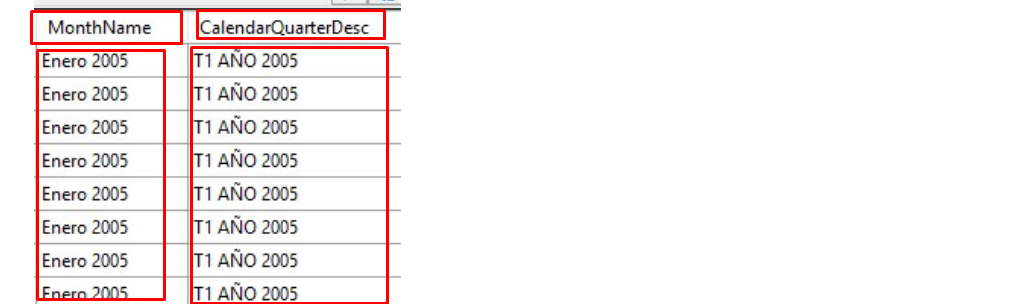
\includegraphics[width=\columnwidth]{images/task6/img3}
	\end{center}	

11. En el panel Tablas, haga clic derecho en DimDate y, a continuación, haga clic en Nuevo cálculo con nombre

12. En el cuadro de diálogo Crear cálculo con nombre, escriba CalendarSemesterDesc en el cuadro Nombre de
columna y, a continuación, escriba el script SQL siguiente en el cuadro Expresión:

	\begin{center}
	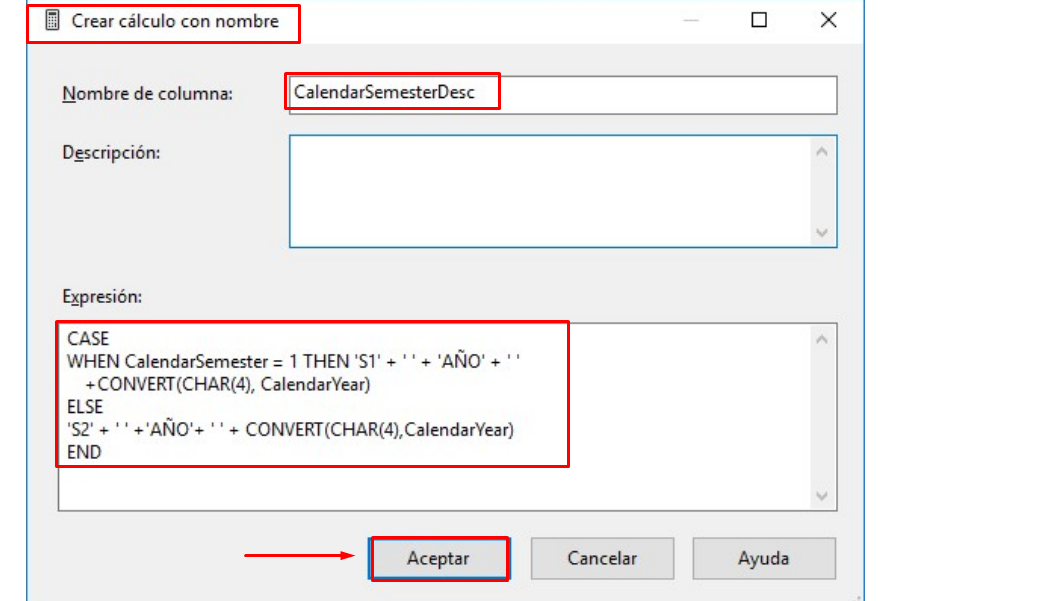
\includegraphics[width=\columnwidth]{images/task6/img4}
	\end{center}	

13. Este script SQL concatena el semestre natural y el año de cada semestre de la tabla en una nueva columna.

14. Haga clic en Aceptar

15. En el menú Archivo del proyecto, haga clic en Guardar todo

16. Haga clic derecho sobre la dimensión DimDate y seleccione la opción Explorar datos y al final de la tabla puede
observar la siguiente información:

	\begin{center}
	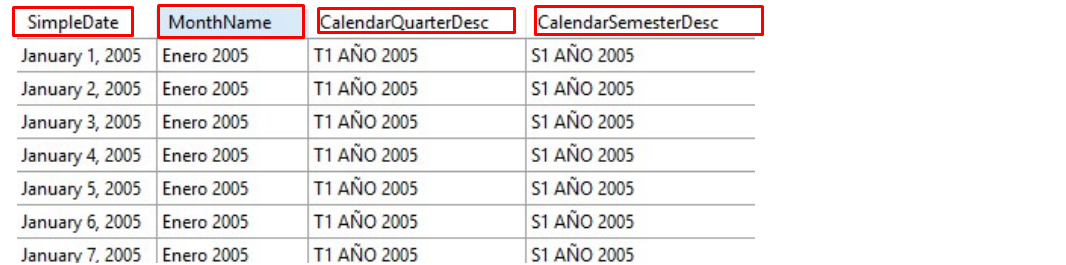
\includegraphics[width=\columnwidth]{images/task6/img5}
	\end{center}	

17. Cerrar todas las pestañas

18. Procesar el cubo, hacer clic en la opción SI, indicando que el cubo ha cambiado desde su última implementación

19. Examinar el cubo

	\begin{center}
	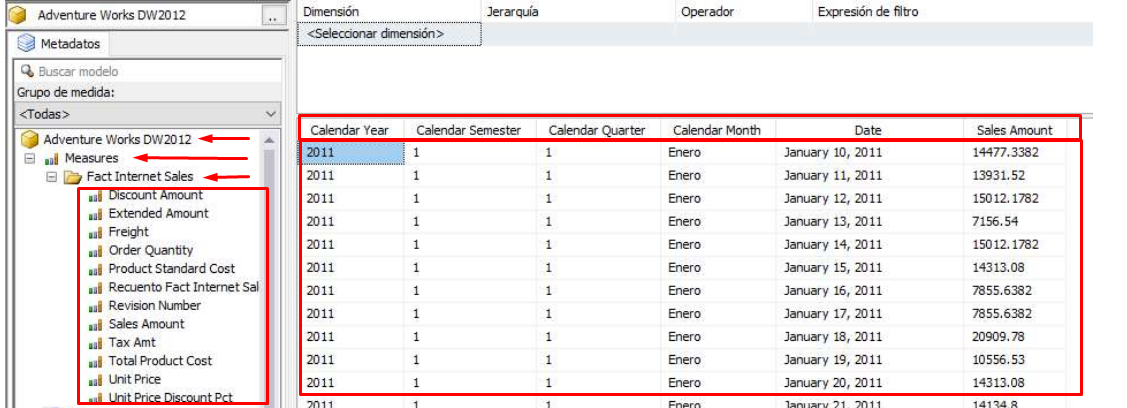
\includegraphics[width=\columnwidth]{images/task6/img6}
	\end{center}	